\chapteropen{Chapter 5: State machines and activity diagrams}{chapter-5}
\markboth{Ch. 5 | Dynamic models}{}


\begin{studycolumns}
\vspace{0pt}
\begin{eli5box}
A traffic light has states such as Red and Green; 'change colour' is an action. A pizza-order workflow has activities such as take order, bake and deliver. Use a state machine to explain one object's changing condition; use an activity diagram to explain how work moves among participants.
\end{eli5box}
\textbf{Answer check:} Model the named object/workflow. Check guards, equality, cancellation, timeouts, retry counts and late replies. A dialog map models interaction/screens. Do not force a final node onto permanent monitoring; do not rename actions as states.
\end{studycolumns}

\subsection*{Visual: choose the diagram that answers the question}
\sectionlabel{h-visual-choose-the-diagram-that-answers-the-question}


\par\smallskip\noindent\begin{minipage}{\linewidth}\centering
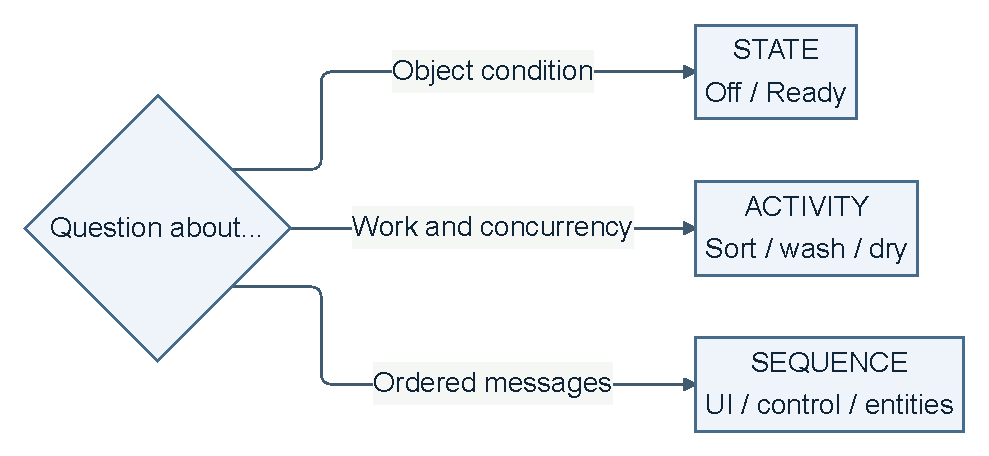
\includegraphics[width=291.18pt]{images/fig-017.pdf}
\captionof{figure}{choose the diagram that answers the question}\end{minipage}\par\smallskip

\begin{studycolumns}
\vspace{0pt}



\needspace{4\baselineskip}
\subsection*{5.1 State machine diagram (a.k.a. statechart, finite state automaton, \textbf{dialog map})}
\sectionlabel{h-51-state-machine-diagram-aka-statechart-finite-state-automaton-dialog-map}
\begin{itemize}
\item Models a system/\allowbreak{}object by the \textbf{states} it can be in.
\item \textbf{State} = a \emph{stable condition} that exists for a period (or all) of time until an \textbf{action/\allowbreak{}event} drives it to another stable state.
\item Finite number of states; transitions determined by previous state and actions.
\item Notation: rounded rectangle, name at top, optional \textbf{entry /\allowbreak{} action}, \textbf{exit /\allowbreak{} action}, \textbf{do /\allowbreak{} activity}.
\item A diagram begins with a \textbf{start node} (filled circle) and ends with an \textbf{end node} --- \textbf{unless} the system loops forever, in which case there is no end node.
\item A transition is \textbf{assumed instantaneous} in response to an event. Full label:
\end{itemize}

\begin{ReferenceCode}
event(arguments) [guard] / action
\end{ReferenceCode}
\textbf{Dialog map} = a state machine used to prototype navigation. Since most UIs show one screen/\allowbreak{}window at a time (a state) with defined conditions to move (transitions), dialog maps:

\begin{itemize}
\item find \textbf{missing or incorrect navigation pathways early}, when they are cheap to fix;
\item spot \textbf{reuse opportunities and redundancies} without premature screen design.
\end{itemize}
\textbf{Worked states:} see the case-specific dialog/state answers in the past papers. A self-transition exits and re-enters its state, so entry actions run again.

\textbf{Action semantics:} do may complete before state exit; entry/exit run on every entry/exit, including re-entry. Decision guards must be mutually exclusive and cover intended cases (or use \code{[else]}).

\needspace{4\baselineskip}
\subsection*{5.2 Activity diagram}
\sectionlabel{h-52-activity-diagram}
\begin{itemize}
\item \textbf{Activity} = execution of one or more basic operations (rounded rectangle).
\item \textbf{Control flow} = arrows.
\item \textbf{Fork} = one input, two or more \textbf{concurrent} outputs (\textbf{thick bar}).
\item \textbf{Join} = two or more flows come together into one (\textbf{thick bar}).
\item \textbf{Decision/\allowbreak{}branch} = one input, several guarded outputs (\textbf{diamond}).
\item \textbf{Merge} = several branches into one (\textbf{diamond}).
\end{itemize}


\needspace{374pt}
\par\smallskip\noindent\begin{minipage}{\linewidth}\centering
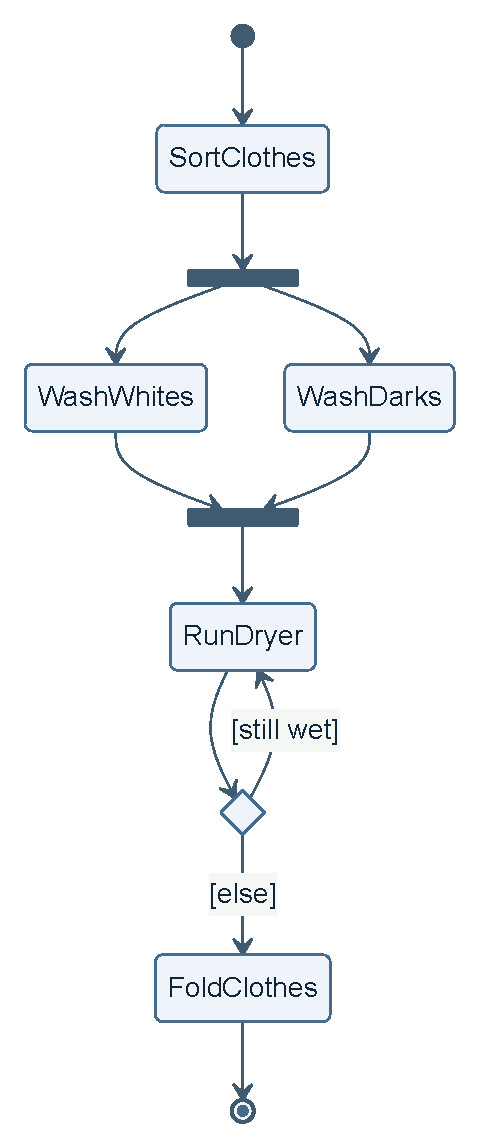
\includegraphics[width=125.48pt]{images/fig-019.pdf}
\captionof{figure}{5.2 Activity diagram}\end{minipage}\par\smallskip


\textbf{UML check:} use action nodes, initial/final nodes and guarded diamonds. A join waits for parallel inputs; a merge rejoins alternatives.
\end{studycolumns}

\Needspace{4\baselineskip}
\subsection*{5.3 State machine vs activity diagram (L6 comparison)}
\sectionlabel{h-53-state-machine-vs-activity-diagram-l6-comparison}


{\fontsize{9}{11}\selectfont
\begin{longtable}{L{\dimexpr 0.23178\linewidth-5.56pt\relax}L{\dimexpr 0.39810\linewidth-9.55pt\relax}L{\dimexpr 0.37012\linewidth-8.88pt\relax}}
\toprule
\rowcolor{ice}\textbf{} & \textbf{\textbf{State machine}} & \textbf{\textbf{Activity}} \\
\midrule\endfirsthead
\toprule\rowcolor{ice}\textbf{} & \textbf{\textbf{State machine}} & \textbf{\textbf{Activity}} \\
\midrule\endhead
\multicolumn{3}{r}{\scriptsize Continued on next page}\\\endfoot
\bottomrule\endlastfoot
Models & The \textbf{states} of a system/\allowbreak{}object and events that move it & The \textbf{workflow of activities} (a flow chart) \\
Node meaning & A stable condition & A unit of work \\
Focus & Event-driven \textbf{reactive} behaviour & Procedural \textbf{control flow}, concurrency \\
Typical use & UI navigation (dialog map), protocol/\allowbreak{}device states & Business process, algorithm, use-case flow \\
\end{longtable}
}


\begin{quote}\small\color{navy}
\textbf{Trap:} fork/\allowbreak{}join are \textbf{bars}; decision/\allowbreak{}merge are \textbf{diamonds}. A diamond for concurrency or a bar for a conditional branch uses the wrong notation.

\end{quote}


\subsection*{5.4 The requirements elicitation \& analysis activity diagram (memorise the loop)}
\sectionlabel{h-54-the-requirements-elicitation--analysis-activity-diagram-memorise-the-loop}



\par\smallskip\noindent\begin{minipage}{\linewidth}\centering
\begin{minipage}[t]{0.488\linewidth}\centering\scriptsize\textbf{1}\par\smallskip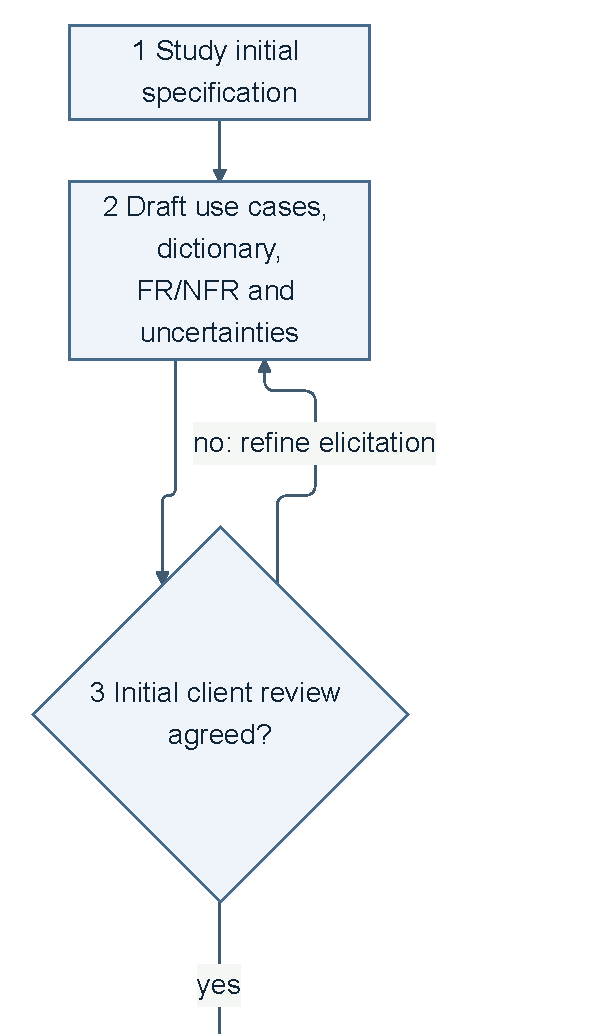
\includegraphics[width=177.48pt]{images/fig-020-compact-1.pdf}\end{minipage}\hfill
\begin{minipage}[t]{0.488\linewidth}\centering\scriptsize\textbf{2}\par\smallskip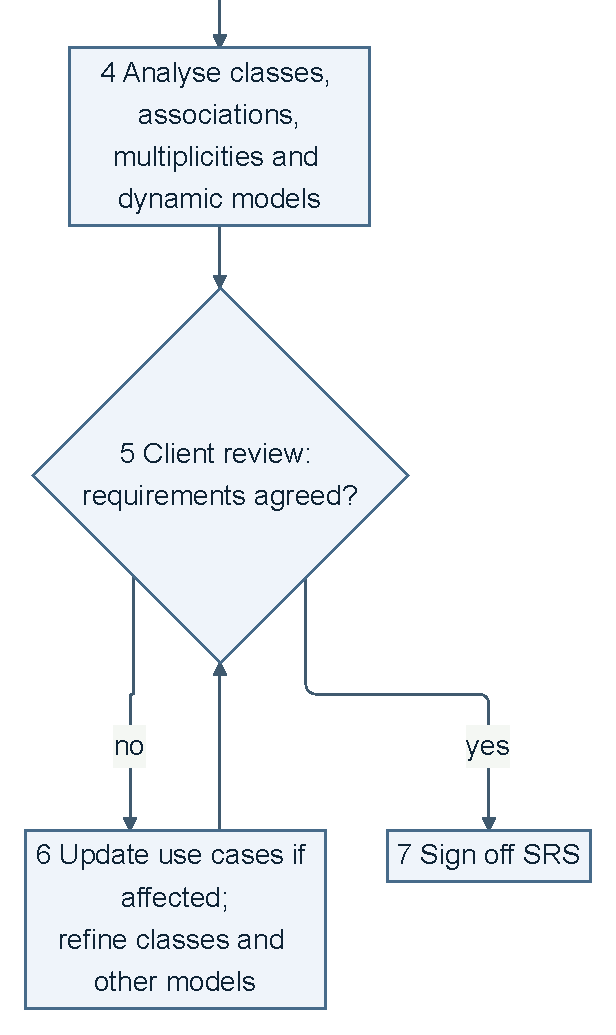
\includegraphics[width=177.48pt]{images/fig-020-compact-2.pdf}\end{minipage}
\captionof{figure}{5.4 The requirements elicitation \& analysis activity diagram --- follow numbered panels; crossing arrows continue.}\end{minipage}\par\smallskip



